\subsubsection{\bf Introduction}
StudentRayleighMonitor is a tool for investigating stationarity non-Gaussianity of input signal $x(t)$
by assuming detector noise distributed the Student-t distribution.
In this assumption, non-Gaussianity is represented by only one parameter, $\nu$, which shows weight of tail of the distribution.
Non-Gaussianity, $\nu$, is computed as the function of time, $t$, and frequency, $f$, from normalized spectrum of $x(t)$.

Normalized spectrogram, $w(t, f)$, of input signal, $x(t)$, is calculated
\begin{align*}
  w(t_i,~f_j) = \frac{ |~{\rm STFT}[x(t)]~| }{S_{\rm 0}(f)},
\end{align*}
where $1\leq i\leq N$, ~$1\leq j\leq M$ and $S_{\rm 0}(f)$ is a normalization factor.
Normalization factor can be estimated
\begin{align*}
  S_{\rm 0}(f) = |~{\rm FFT}[x(t)]~|.
\end{align*}
P-quantile value of input signal is calculated from normalized spectrogram as the function of time and frequency,
$Q_{P}(t_k, f_l)$ where $1\leq k\leq N/n$, $1\leq l\leq M/m$, $n(k-1)+1\leq i\leq nk$ ,
$m(l-1)-1\leq j\leq ml$, $n = {\rm d}t/{\rm d}t_{\rm fft}$ and $m = {\rm d}f/{\rm d}f_{\rm fft} = {\rm d}f~{\rm d}t_{\rm fft}$

On the other hand, theoretical quantile value in the Student-t noise case can be described
\begin{align*}
  Q_{\rm sr}(\sigma,\nu;P) = \sigma\sqrt{\frac{\nu(1-(1-P)^{2/\nu})}{(1-P)^{2/\nu}}}
\end{align*}

Degree of non-Gaussianity $\nu$ is calculated from P-quantile value of data and theoretical quantile value.
\begin{align*}
  \nu(t_k, f_l) = \mathop{\rm arg~min}\limits_{\nu} | Q_{P=P_0}(t_k,f_l) - Q_{\rm sr}(\sigma,\nu;P=P_0)|
\end{align*}

\subsubsection{{\bf Function:} studentRayleighMonWaveData}
{\tt studentRayleighMonWaveData p secfft chunck dt df x0 xt\\}

This function compute the non-Gaussianity, $\nu$, of the input signal, $x(t)$, as the function of time, $t$, and frequency, $f$.
The arguments are:
\begin{itemize}
\item {\tt p}: Input. The dimensionless p-value ($0 \leq p \leq 1$).
\item {\tt secfft}: Input. The data length for short time Fourier transform in seconds.
\item {\tt chunck}: Input. The data length for estimating $\nu(f)$ in seconds. ({\tt secfft} $\leq$ {\tt chunck})
\item {\tt dt}: Input. The time resolution of $\nu(t,~f)$ in seconds.
\item {\tt df}: Input. The frequency resolution of $\nu(t, f)$ in Hertz
\item {\tt x0}: Input. The time series signal for estimating averaged spectrum
\item {\tt xt}: Input. The time series for estimating $\nu(t,~f)$
\item {\tt nu}: Output. The dimensionless non-Gaussian parameter $\nu(t,~f)$.
\end{itemize}

\subsubsection{{\bf Example:} studentRayleighMon}
This program calculates the $\nu(t, f)$ of the input signals.\\

{\noindent \bf Typical usage:} {\tt studentRayleighMon param.conf file.lst}
{\footnotesize
\begin{verbatim}
  import Data.Maybe (catMaybes)
  import System.Environment (getArgs)

  import HasKAL.DetectorUtils.Detector (Detector(..))
  import HasKAL.FrameUtils.Function (readFrameWaveData')
  import HasKAL.Misc.ConfFile (readFileList, readConfFile)
  import HasKAL.MonitorUtils.SRMon.StudentRayleighMon (studentRayleighMonWaveData)
  import HasKAL.PlotUtils.HROOT.PlotGraph3D
  import HasKAL.WaveUtils.Data (WaveData(..))
  import HasKAL.WaveUtils.Function (catWaveData)

  main = do
    {-- arg check --}
    args <- getArgs
    (conf, lst) <- case length args of
                    2 -> return (args!!0, args!!1)
                    _ -> error "Usage: rayleighMon conffile filelist"

    {-- read param --}
    filelist <- readFileList lst                                                                                    
    ([ch, q, dtfft, dt, lap, df], _) <- readConfFile conf ["channel", "quantile", "dtfft"
                                                          , "dt", "overlap", ``df"] []

    {-- read data --}
    mbWd <- mapM (readFrameWaveData' KAGRA ch) filelist
    let wd = case catMaybes mbWd of
              [] -> error "Can't find data"
              xs -> catWaveData xs

    {-- main --}
    let result = studentRayleighMonWaveData (read q) (read dtfft)
                    (read dt) (read dt - read lap) (read df) wd wd
        title = ch ++ ": " ++ (show . fst . startGPSTime $ wd)
                   ++ " ~ " ++ (show . fst . stopGPSTime $ wd)
    histgram2dM Linear COLZ ("time [s]", "frequency [Hz]", "nu")
       title "X11" ((0,0),(0,0)) $ result

\end{verbatim}
}

{\noindent \bf Param file format:} {\tt param.conf}
{\footnotesize
\begin{verbatim}
  channel: X1:HOGE-XX  # channel name
  quantile: 0.95       # dimensionless p-value
  dtfft: 1             # data length for STFT in seconds
  dt: 128              # time resolution of \nu(t,f) in seconds
  overlap: 124         # data overlap in seconds
  df: 16               # frequency resolution of \nu(t,f) in Hertz

\end{verbatim}
}

{\noindent \bf List file format:} {\tt file.lst}
{\footnotesize
\begin{verbatim}
  /path/to/framefile/a.gwf
  /path/to/framefile/b.gwf

\end{verbatim}
}

\begin{figure}[t]
  \begin{center}
    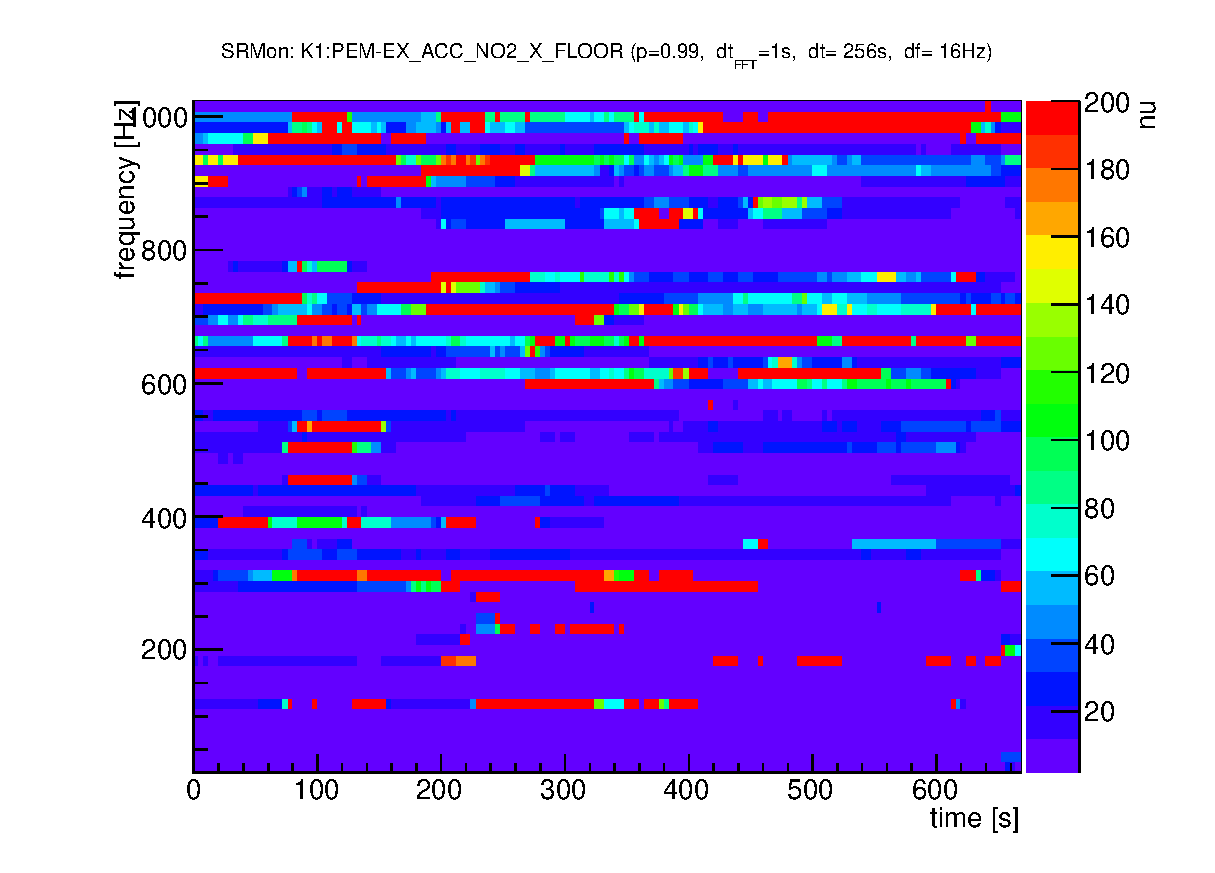
\includegraphics[width=0.9\hsize]{fig/StudentRayleighMon/sample1.eps}
    \caption{sample plot of studentRayleighMonitor}
  \end{center}
\end{figure}

{\noindent \small contact person: Takahiro Yamamoto (\tt yamamoto@yukimura.hep.osaka-cu.ac.jp)}

